\documentclass[10pt]{beamer}
\usepackage[english]{babel}
\usepackage[utf8]{inputenc}
\usepackage[T1]{fontenc}
\usepackage{helvet}

%-------------------------------------------------------
% INFORMATION IN THE TITLE PAGE
%-------------------------------------------------------

\newcommand{\cstitle}{\textbf{Bioinformatics}}
\subtitle[]{Introduction to Bioinformatics}
\newcommand{\cscourseCode}{1005155}
\newcommand{\csauthor}{MSc. Vicente Machaca Arceda}
\institute[UNSA]{Universidad Nacional de San Agustín de Arequipa}
\newcommand{\csemail}{vmachacaa@unsa.edu.pe}
\newcommand{\instituteabr}{UNSA}
\newcommand{\nameUp}{ICC Fase 1}
\date{\today}
\title[\cscourseCode]{\cstitle}
\author{\csauthor}
%%%%%%%%%%%%%%%%%

%-------------------------------------------------------
% CHOOSE THE THEME
%-------------------------------------------------------
\def\mycmd{0} % CS THEME
%\def\mycmd{1} % MYTHEME
%-------------------------------------------------------

\if\mycmd1
	\usetheme[]{Feather}
	\newcommand{\chref}[2]{	\href{#1}{{\usebeamercolor[bg]{Feather}#2}} }
\else
	\usepackage{csformat}
\fi

\newcommand{\1}{
        	\setbeamertemplate{background}{
        		
\includegraphics[width=\paperwidth,height=\paperheight]{img/1}
        		\tikz[overlay] \fill[fill opacity=0.75,fill=white] (0,0) rectangle (-\paperwidth,\paperheight);
        	}
}



%-------------------------------------------------------
% THE BODY OF THE PRESENTATION
%-------------------------------------------------------

\begin{document}


\AtBeginSection[]
{
    \begin{frame}
        \frametitle{Table of Contents}
        \tableofcontents[currentsection]
    \end{frame}
}


%-------------------------------------------------------
% THE TITLEPAGE
%-------------------------------------------------------

\if\mycmd1 % MY THEME
	\1{
	\begin{frame}[plain,noframenumbering] 
		\titlepage 
	\end{frame}}

\else % CS THEME
	\maketitle
\fi


%-------------------------------------------------------
%-------------------------------------------------------
\begin{frame}{Overview}
	\tableofcontents
\end{frame}
%-------------------------------------------------------
%-------------------------------------------------------


\section{Introduction}

%%%%%%%%%%%%%%%%%%%%%%%%%%%%%%%%%%%%%%%%%%%%%%%%%%%%%%%%
\subsection{Objectives}
%%%%%%%%%%%%%%%%%%%%%%%%%%%%%%%%%%%%%%%%%%%%%%%%%%%%%%%%

%-------------------------------------------------------
%-------------------------------------------------------
\begin{frame}{Objectives}{}
	\begin{itemize}
		\item<1-> Understand what is Bioinformatics, Computer Biology and Computation Molecular Biology. 
		\item<2-> Learn the areas of research in Bioinformatics.
	\end{itemize}
\end{frame}
%-------------------------------------------------------
%-------------------------------------------------------

%%%%%%%%%%%%%%%%%%%%%%%%%%%%%%%%%%%%%%%%%%%%%%%%%%%%%%%%
\subsection{Motivation}
%%%%%%%%%%%%%%%%%%%%%%%%%%%%%%%%%%%%%%%%%%%%%%%%%%%%%%%%

%-------------------------------------------------------
%-------------------------------------------------------
\begin{frame}{Motivation}{What microorganism live in our armpits or in our mouths?}
	\begin{figure}[]
		\centering
		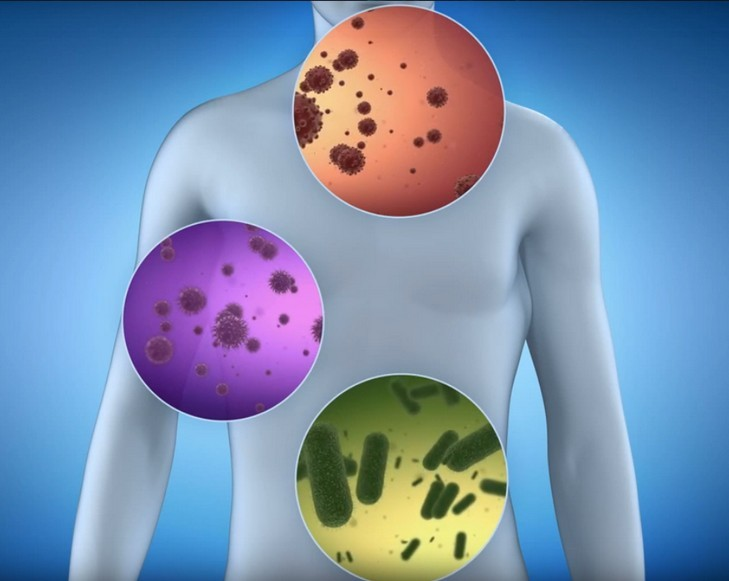
\includegraphics[width=\textwidth,height=0.7\textheight,keepaspectratio]{img/introduction/mot1.jpg}
		\label{img:mot1}
		\caption{What microorganism live in our armpits or in our mouths?}
	\end{figure}
\end{frame}
%-------------------------------------------------------
%-------------------------------------------------------

%-------------------------------------------------------
%-------------------------------------------------------
\begin{frame}{Motivation}{Is there a kindness gene?
	}
	\begin{figure}[]
		\centering
		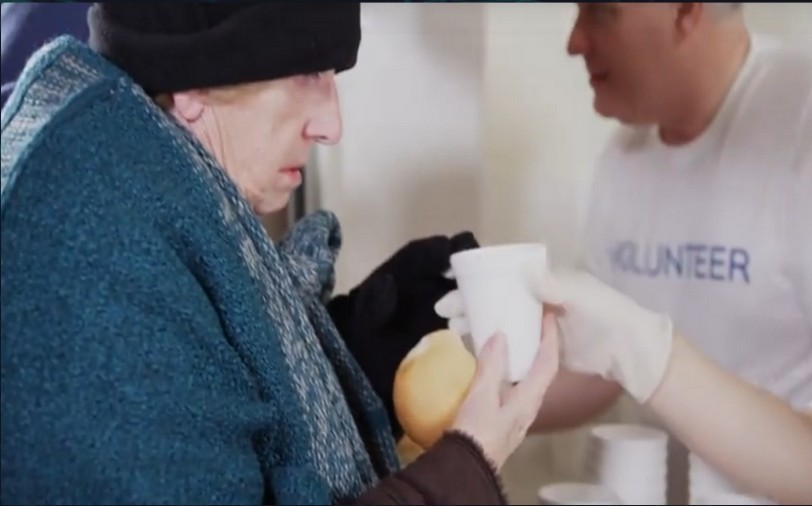
\includegraphics[width=\textwidth,height=0.7\textheight,keepaspectratio]{img/introduction/mot2.jpg}
		\label{img:mot2}
		\caption{Is there a kindness gene?}
	\end{figure}
\end{frame}
%-------------------------------------------------------
%-------------------------------------------------------

%-------------------------------------------------------
%-------------------------------------------------------
\begin{frame}{Motivation}{Why a person has cancer?}
	\begin{figure}[]
		\centering
		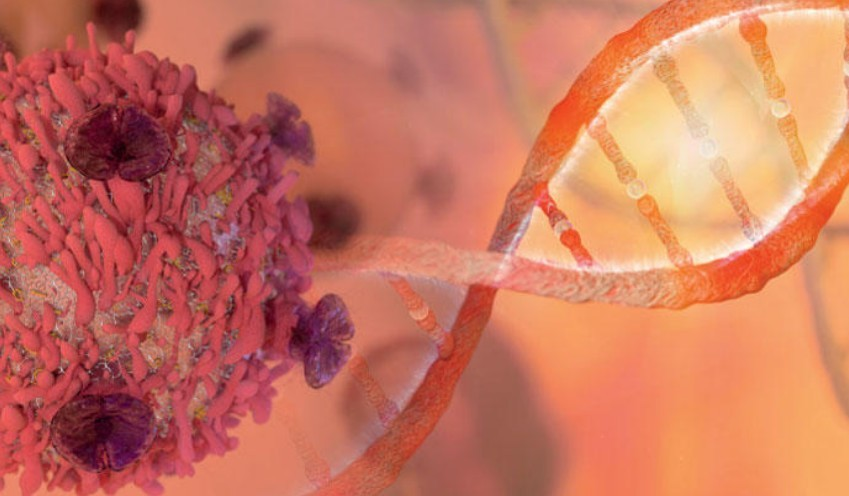
\includegraphics[width=\textwidth,height=0.6\textheight,keepaspectratio]{img/introduction/mot3.jpg}
		\label{img:mot2}
		\caption{Why a person has cancer?}
	\end{figure}
\end{frame}
%-------------------------------------------------------
%-------------------------------------------------------

%-------------------------------------------------------
%-------------------------------------------------------
\begin{frame}{Motivation}{Why some medicines no work in some persons?}
	\begin{figure}[]
		\centering
		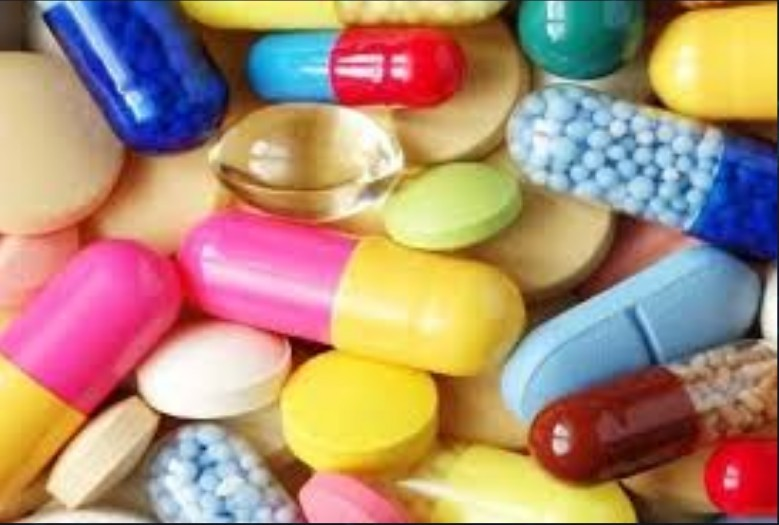
\includegraphics[width=\textwidth,height=0.6\textheight,keepaspectratio]{img/introduction/mot4.jpg}
		\label{img:mot2}
		\caption{Why some medicines no work in some persons?}
	\end{figure}
\end{frame}
%-------------------------------------------------------
%-------------------------------------------------------

%-------------------------------------------------------
%-------------------------------------------------------
\begin{frame}{Motivation}{Treatment Development}
	\begin{figure}[]
		\centering
		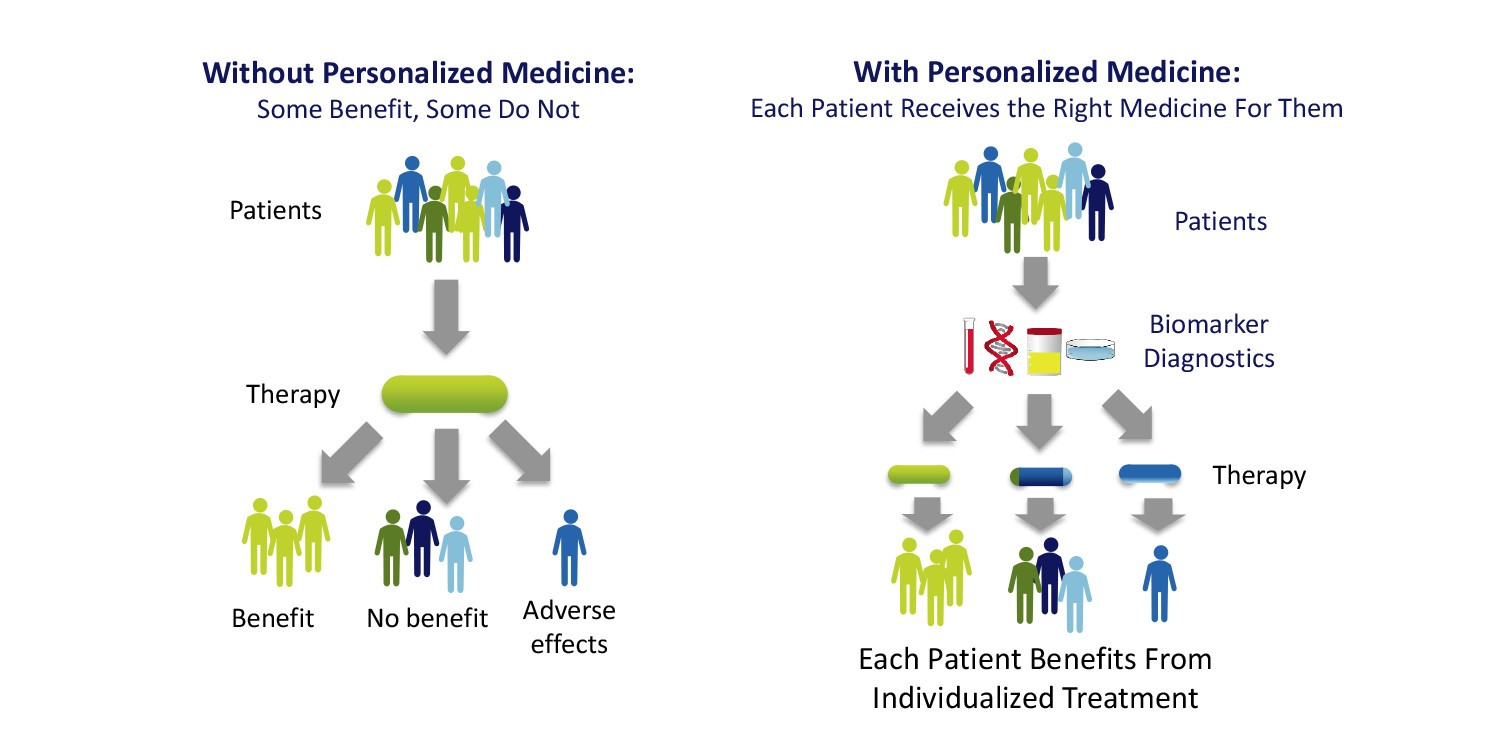
\includegraphics[width=\textwidth,height=0.7\textheight,keepaspectratio]{img/introduction/mot5.jpg}
		\label{img:mot2}
		\caption{Personalized Medicine: New Approach to Treatment of Disease}
	\end{figure}
\end{frame}
%-------------------------------------------------------
%-------------------------------------------------------

%%%%%%%%%%%%%%%%%%%%%%%%%%%%%%%%%%%%%%%%%%%%%%%%%%%%%%%%
\subsection{What is Bioinformatics?}
%%%%%%%%%%%%%%%%%%%%%%%%%%%%%%%%%%%%%%%%%%%%%%%%%%%%%%%%

%-------------------------------------------------------
\begin{frame}{Introduction}{What is Bioinformatics?}
	%-------------------------------------------------------
	
	According to Luscombe et al.: \textbf{Bioinformatics} involves the technology that uses computers for storage, retrieval, manipulation, and distribution of information related to biological macromolecules such as DNA, RNA, and proteins \cite{luscombe2001bioinformatics}.
	
\end{frame}

%-------------------------------------------------------
%-------------------------------------------------------
\begin{frame}{Introduction}{Bioinformatics vs Computational Biology}
	\textbf{Bioinformatics} is limited to sequence, structural, and functional analysis of genes and genomes and their corresponding products and is often considered \textbf{Computational
		molecular biology}. However, \textbf{Computational Biology} encompasses all biological areas that involve computation \cite{xiong2006essential}.
\end{frame}
%-------------------------------------------------------
%-------------------------------------------------------

%-------------------------------------------------------
%-------------------------------------------------------
\begin{frame}{Introduction}{Genomics}
	\textbf{Genomics} is the study of whole genomes of organisms. Genomics uses a combination of recombinant DNA, DNA sequencing methods, and bioinformatics to sequence, assemble, and analyse the structure and function of genomes. It differs from classical \textbf{Genetics} in that it study genes and their heredity meanwhile Genomics study the whole genome  \cite{archibald2018genomics}.
\end{frame}
%-------------------------------------------------------
%-------------------------------------------------------


%-------------------------------------------------------
%-------------------------------------------------------
\begin{frame}{Motivation}{Areas Bioinformaics can help with}
	\begin{columns}
		\begin{column}{0.68\textwidth}
			
			\begin{figure}[]
				\centering
				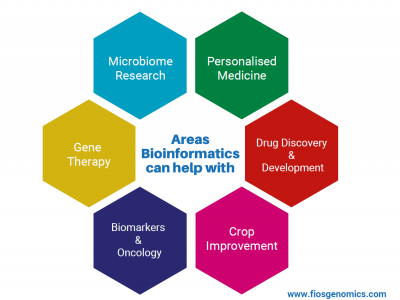
\includegraphics[width=\textwidth,height=0.7\textheight,keepaspectratio]{img/introduction/bio_areas.png}
				\label{img:mot2}
				\caption{Areas Bioinformaics can help with.}
			\end{figure}
		\end{column}
		\begin{column}{0.28\textwidth}
			\textbf{Microbiome} study the genetic material of microbes, bacteria, fungi, etc.
		\end{column}
	\end{columns}
\end{frame}
%-------------------------------------------------------
%-------------------------------------------------------

%-------------------------------------------------------
%-------------------------------------------------------
\begin{frame}{Motivation}{Areas Bioinformaics can help with}
	\begin{columns}
		\begin{column}{0.68\textwidth}
			
			\begin{figure}[]
				\centering
				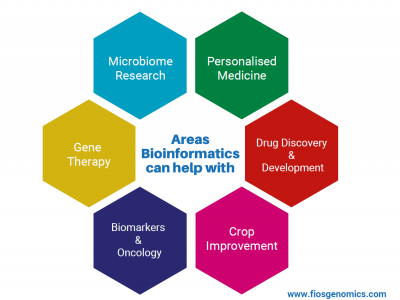
\includegraphics[width=\textwidth,height=0.7\textheight,keepaspectratio]{img/introduction/bio_areas.png}
				\label{img:mot2}
				\caption{Areas Bioinformaics can help with.}
			\end{figure}
		\end{column}
		\begin{column}{0.28\textwidth}
			\textbf{Personalized medicine} has the potential to tailor therapy with the best response and highest safety margin to ensure better patient care.
		\end{column}
	\end{columns}
\end{frame}
%-------------------------------------------------------
%-------------------------------------------------------

%-------------------------------------------------------
%-------------------------------------------------------
\begin{frame}{Motivation}{Areas Bioinformaics can help with}
	\begin{columns}
		\begin{column}{0.68\textwidth}
			
			\begin{figure}[]
				\centering
				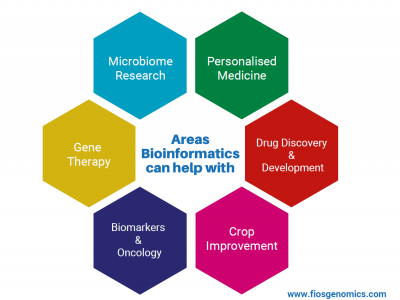
\includegraphics[width=\textwidth,height=0.7\textheight,keepaspectratio]{img/introduction/bio_areas.png}
				\label{img:mot2}
				\caption{Areas Bioinformaics can help with.}
			\end{figure}
		\end{column}
		\begin{column}{0.28\textwidth}
			\textbf{Drug descovery} is the process through which potential new medicines are identified.
		\end{column}
	\end{columns}
\end{frame}
%-------------------------------------------------------
%-------------------------------------------------------

%-------------------------------------------------------
%-------------------------------------------------------
\begin{frame}{Motivation}{Areas Bioinformaics can help with}
	\begin{columns}
		\begin{column}{0.68\textwidth}
			
			\begin{figure}[]
				\centering
				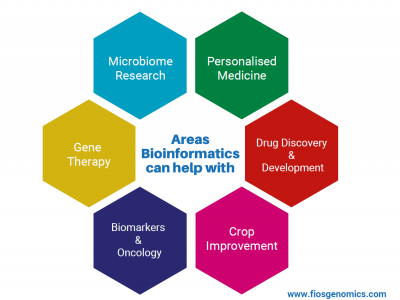
\includegraphics[width=\textwidth,height=0.7\textheight,keepaspectratio]{img/introduction/bio_areas.png}
				\label{img:mot2}
				\caption{Areas Bioinformaics can help with.}
			\end{figure}
		\end{column}
		\begin{column}{0.28\textwidth}
			\textbf{Crop improvement} help to produce stronger, more drought, disease and insect resistant crops.
		\end{column}
	\end{columns}
\end{frame}
%-------------------------------------------------------
%-------------------------------------------------------

%-------------------------------------------------------
%-------------------------------------------------------
\begin{frame}{Motivation}{Areas Bioinformaics can help with}
	\begin{columns}
		\begin{column}{0.68\textwidth}
			
			\begin{figure}[]
				\centering
				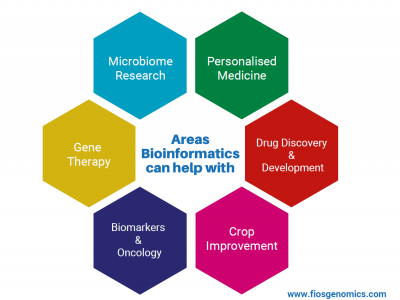
\includegraphics[width=\textwidth,height=0.7\textheight,keepaspectratio]{img/introduction/bio_areas.png}
				\label{img:mot2}
				\caption{Areas Bioinformaics can help with.}
			\end{figure}
		\end{column}
		\begin{column}{0.28\textwidth}
			\textbf{Biomarkers \& oncology} could be used as screening/early detection tool of cancer  diagnostic and prognostic.
		\end{column}
	\end{columns}
\end{frame}
%-------------------------------------------------------
%-------------------------------------------------------


%-------------------------------------------------------
%-------------------------------------------------------
\begin{frame}{Motivation}{Areas Bioinformaics can help with}
	\begin{columns}
		\begin{column}{0.68\textwidth}
			
			\begin{figure}[]
				\centering
				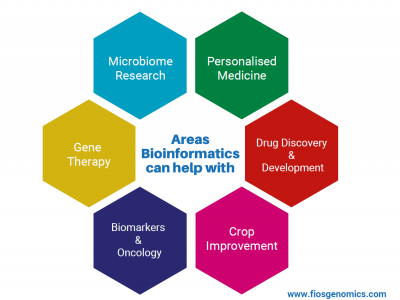
\includegraphics[width=\textwidth,height=0.7\textheight,keepaspectratio]{img/introduction/bio_areas.png}
				\label{img:mot2}
				\caption{Areas Bioinformaics can help with.}
			\end{figure}
		\end{column}
		\begin{column}{0.28\textwidth}
			\textbf{Gene therapy} is an experimental technique that uses genes to treat or prevent disease. In the future, this technique could insert a gene into a patient's cells instead of using drugs or surgery.
		\end{column}
	\end{columns}
\end{frame}
%-------------------------------------------------------
%-------------------------------------------------------

%-------------------------------------------------------
%-------------------------------------------------------
\begin{frame}[allowframebreaks]
	\frametitle{References}
	%\bibliographystyle{amsalpha}
	\bibliographystyle{IEEEtran}
	\bibliography{bibliography.bib}
\end{frame}
%-------------------------------------------------------
%-------------------------------------------------------



%-------------------------------------------------------
%-------------------------------------------------------
\if\mycmd1 % MY THEME
\1{
	{\1
		\begin{frame}[plain,noframenumbering]
			\finalpage{Thank you}
		\end{frame}}
	\else % CS THEME
	
\fi
%-------------------------------------------------------
%-------------------------------------------------------
	

\end{document}